\chapter{Classification results evaluation} \label{chapt4}
\section{Base line model} \label{sect4_2}
It is a common knowledge that RNN based neural networks shows the best performance for the text based problems. For my goal, I used Bidirectional Long-Short Term Memory (bi-LSTM) model with 100 ... HERE DESCRIBE MORE ABOUT PARAMETERS 


\begin{figure}[ht] 
	\center
	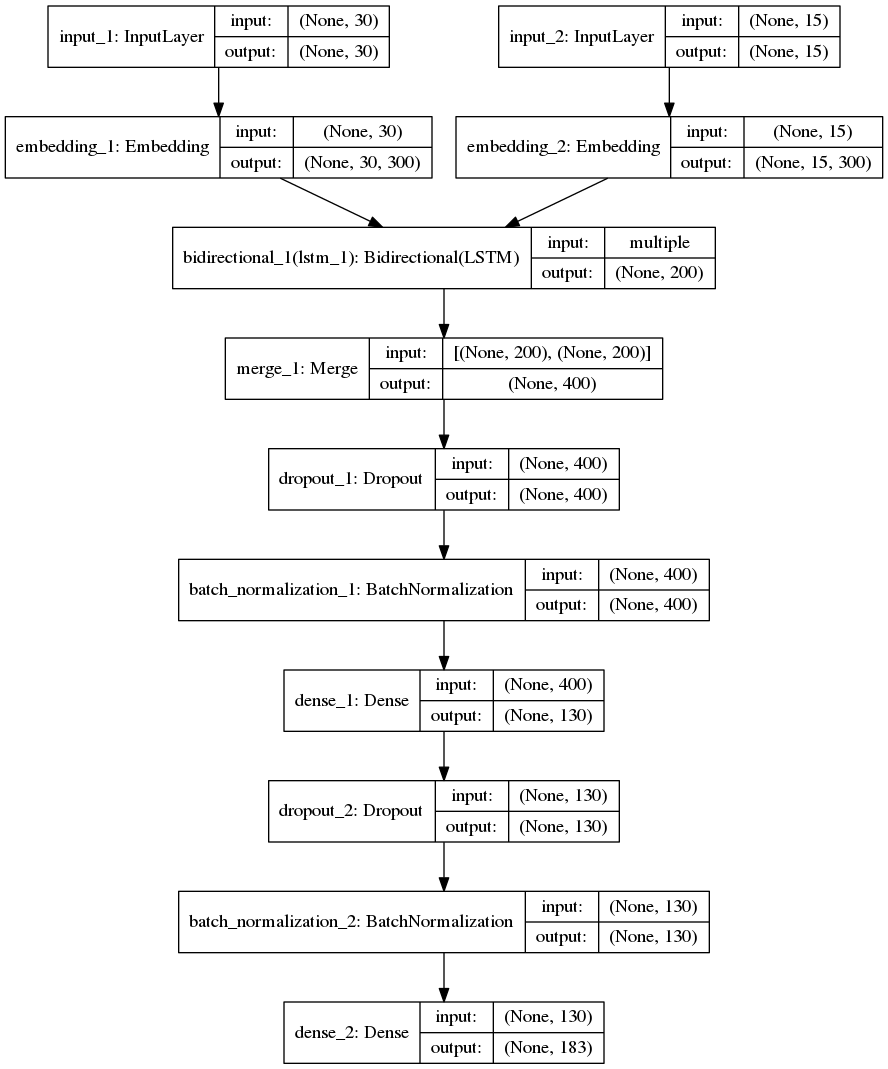
\includegraphics [scale=0.4] {part4/bilstm_architecture.png}
	\label{img:part4-bilstm}  
	\caption{Architectures of Bi-LSTM models with 100 units } 
\end{figure}



top\_k\_categorical\_accuracy


\begin{figure}[ht]
	\begin{minipage}[ht]{1\linewidth}
		\center{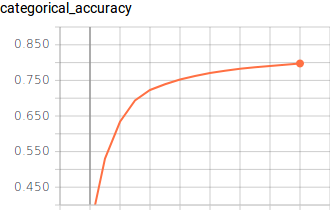
\includegraphics[width=0.5\linewidth]{part4/bilstm_train_category_accuracy}}
	\end{minipage}
	\hfill
	\begin{minipage}[ht]{1\linewidth}
		\center{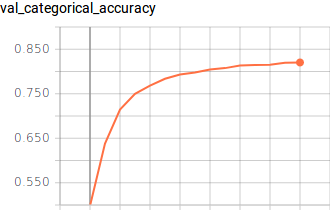
\includegraphics[width=0.5\linewidth]{part4/bilstm_val_category_accuracy}}
	\end{minipage}
	\caption{Models train and validation categorical accuracy by epochs}
	\label{img:categorical_accuracy}  
\end{figure}

\begin{figure}[ht]
	\begin{minipage}[ht]{1\linewidth}
		\center{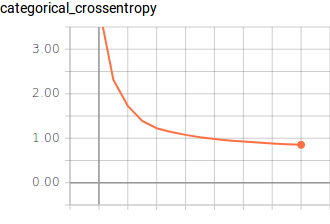
\includegraphics[width=0.5\linewidth]{part4/bilstm_train_category_crossentropy}}
	\end{minipage}
	\hfill
	\begin{minipage}[ht]{1\linewidth}
		\center{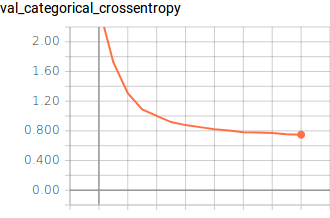
\includegraphics[width=0.5\linewidth]{part4/bilstm_val_category_crossentropy}}
	\end{minipage}
	\caption{Models train and validation category crossentropy by epochs}
	\label{img:category_crossentropy}  
\end{figure}

\begin{figure}[ht]
	\begin{minipage}[ht]{1\linewidth}
		\center{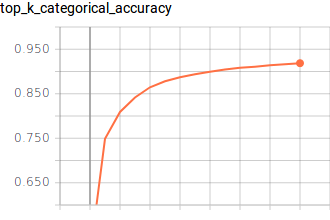
\includegraphics[width=0.5\linewidth]{part4/bilstm_train_top_k_accuracy}}
	\end{minipage}
	\hfill
	\begin{minipage}[ht]{1\linewidth}
		\center{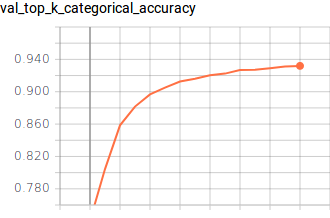
\includegraphics[width=0.5\linewidth]{part4/bilstm_val_top_k_accuracy}}
	\end{minipage}
	\caption{Models train and validation top k accuracy by epochs}
	\label{img:category_crossentropy}  
\end{figure}

\begin{figure}[ht] 
	\center
	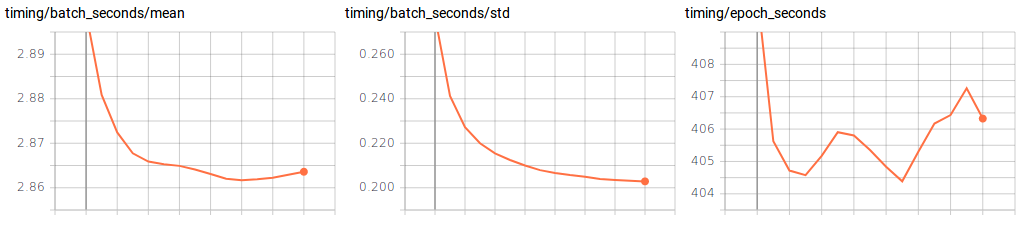
\includegraphics [scale=0.5] {part4/bilstm_timing}
	\caption{Models batch time by epochs} 
	\label{img:bilstm_timing}  
\end{figure}


\begin{figure}[ht]
	\begin{minipage}[ht]{1\linewidth}
		\center{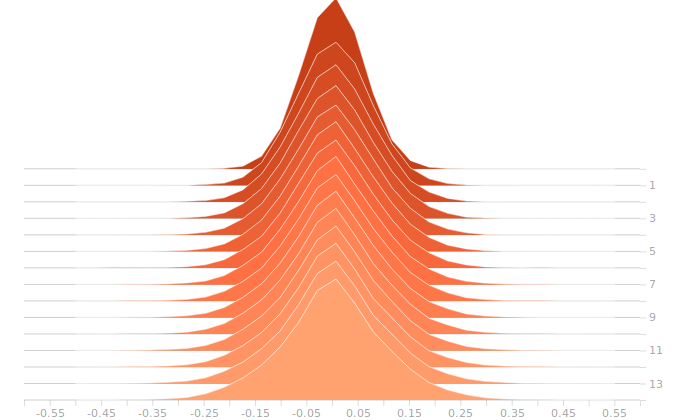
\includegraphics[width=0.5\linewidth]{part4/bilstm_forward_lstm_1_recurrent_kernel_0} \\ а}
	\end{minipage}
	\hfill
	\begin{minipage}[ht]{1\linewidth}
		\center{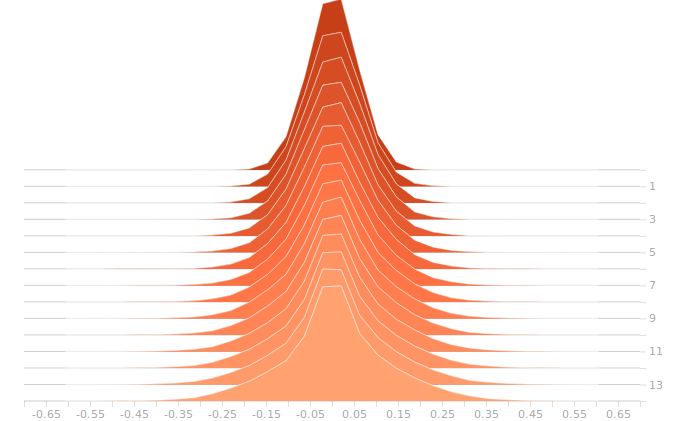
\includegraphics[width=0.5\linewidth]{part4/bilstm_backward_lstm_1_recurrent_kernel_0} \\ b}
	\end{minipage}
	\caption{Bi-LSTM 100 units. Histogram of output from forward recurrent layers (a); histogram of weights from backward recurrent layers (b)}
	\label{img:category_crossentropy}  
\end{figure}


\begin{figure}[ht] 
	\center
	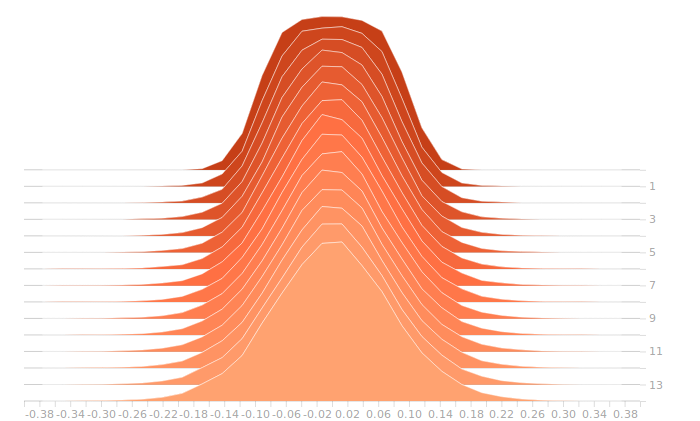
\includegraphics [scale=0.5] {part4/bilstm_dense}
	\caption{Bi-LSTM 100 units. Histogram of weights from first FFNN layer.} 
	\label{img:bilstm_dense}  
\end{figure}

\begin{figure}[ht] 
	\center
	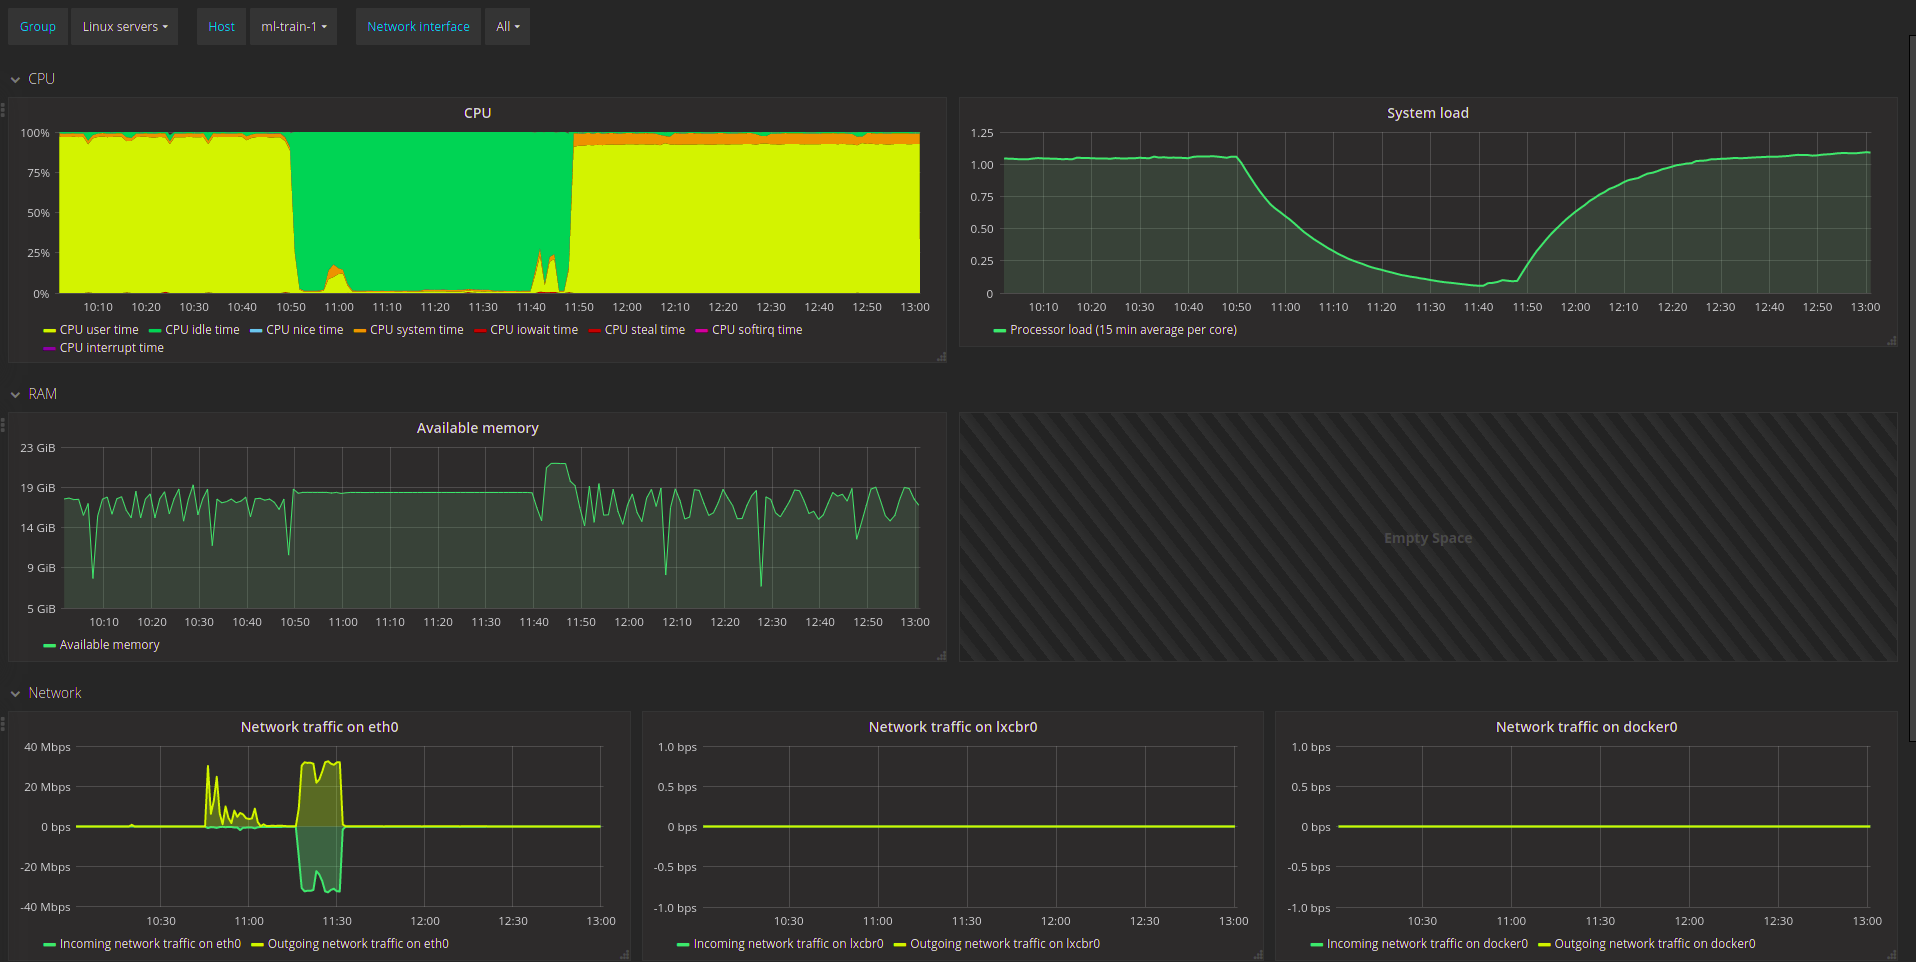
\includegraphics [scale=0.5] {part4/resources_BILSTM}
	\caption{CPU resources which were used while training Bi-LSTM NN.} 
	\label{img:resources_BILSTM}  
\end{figure}

\section{Hyper-parameters fine tuning} \label{sect4_2}


